\documentclass[14pt]{extbook}
\usepackage{multicol, enumerate, enumitem, hyperref, color, soul, setspace, parskip, fancyhdr} %General Packages
\usepackage{amssymb, amsthm, amsmath, latexsym, units, mathtools} %Math Packages
\everymath{\displaystyle} %All math in Display Style
% Packages with additional options
\usepackage[headsep=0.5cm,headheight=12pt, left=1 in,right= 1 in,top= 1 in,bottom= 1 in]{geometry}
\usepackage[usenames,dvipsnames]{xcolor}
\usepackage{dashrule}  % Package to use the command below to create lines between items
\newcommand{\litem}[1]{\item#1\hspace*{-1cm}\rule{\textwidth}{0.4pt}}
\pagestyle{fancy}
\lhead{Progress Quiz 8}
\chead{}
\rhead{Version B}
\lfoot{5493-4176}
\cfoot{}
\rfoot{Summer C 2021}
\begin{document}

\begin{enumerate}
\litem{
Choose the graph of the equation below.\[ f(x) = \frac{-1}{x - 3} + 1 \]\begin{enumerate}[label=\Alph*.]
\begin{multicols}{2}\item 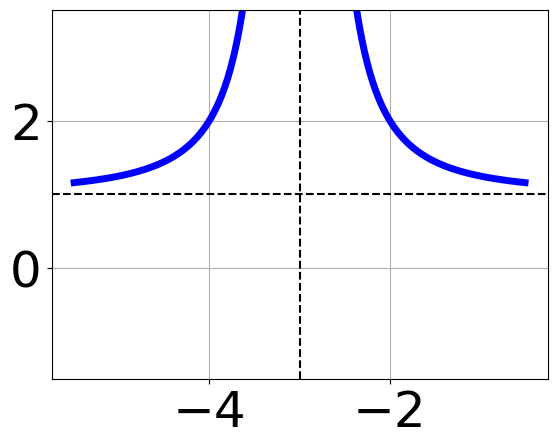
\includegraphics[width = 0.3\textwidth]{../Figures/rationalEquationToGraphCopyAB.png}\item 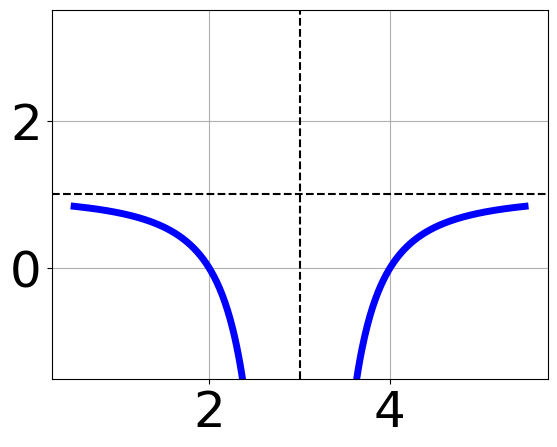
\includegraphics[width = 0.3\textwidth]{../Figures/rationalEquationToGraphCopyBB.png}\item 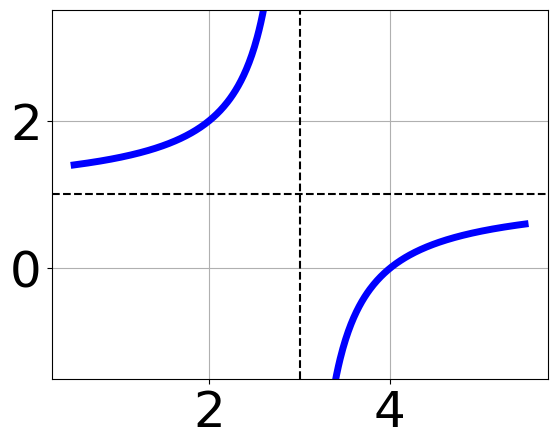
\includegraphics[width = 0.3\textwidth]{../Figures/rationalEquationToGraphCopyCB.png}\item 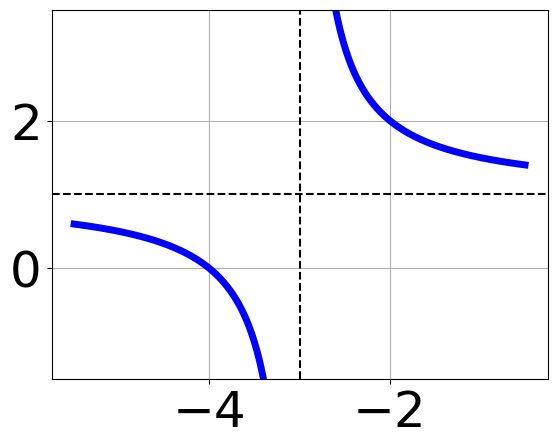
\includegraphics[width = 0.3\textwidth]{../Figures/rationalEquationToGraphCopyDB.png}\end{multicols}\item None of the above.
\end{enumerate} }
\litem{
Solve the rational equation below. Then, choose the interval(s) that the solution(s) belongs to.\[ \frac{-3}{-9x + 9} + 2 = \frac{9}{81x -81} \]\begin{enumerate}[label=\Alph*.]
\item \( \text{All solutions lead to invalid or complex values in the equation.} \)
\item \( x \in [0.89,1.89] \)
\item \( x_1 \in [-0.8, 0.5] \text{ and } x_2 \in [-1.11,2.89] \)
\item \( x \in [-2.8,-0.5] \)
\item \( x_1 \in [-2.8, -0.5] \text{ and } x_2 \in [-1.11,2.89] \)

\end{enumerate} }
\litem{
Choose the graph of the equation below.\[ f(x) = \frac{-1}{x + 2} + 2 \]\begin{enumerate}[label=\Alph*.]
\begin{multicols}{2}\item 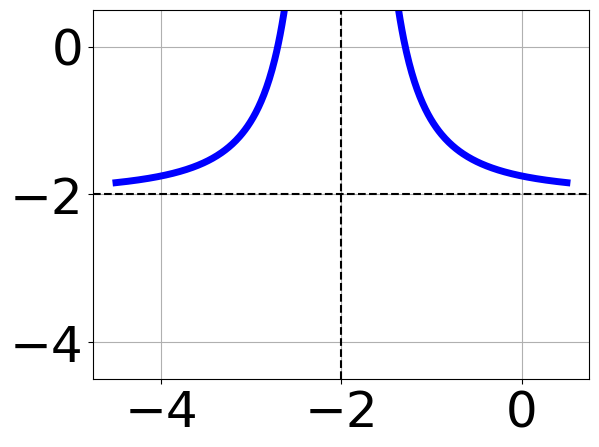
\includegraphics[width = 0.3\textwidth]{../Figures/rationalEquationToGraphAB.png}\item 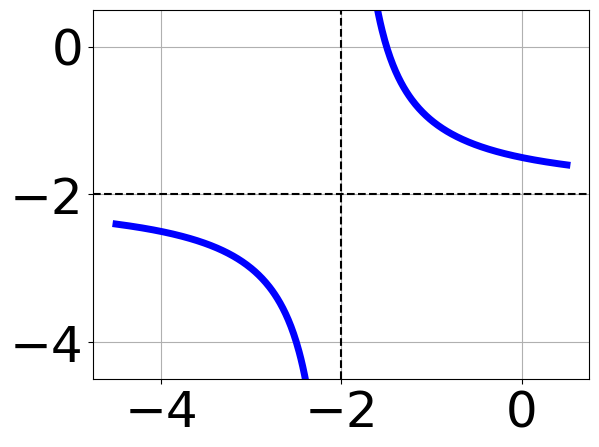
\includegraphics[width = 0.3\textwidth]{../Figures/rationalEquationToGraphBB.png}\item 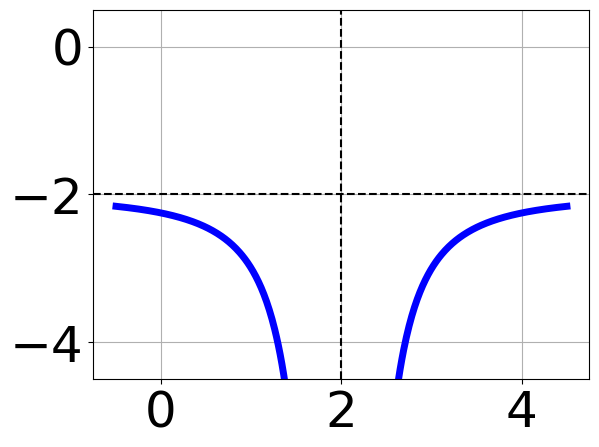
\includegraphics[width = 0.3\textwidth]{../Figures/rationalEquationToGraphCB.png}\item 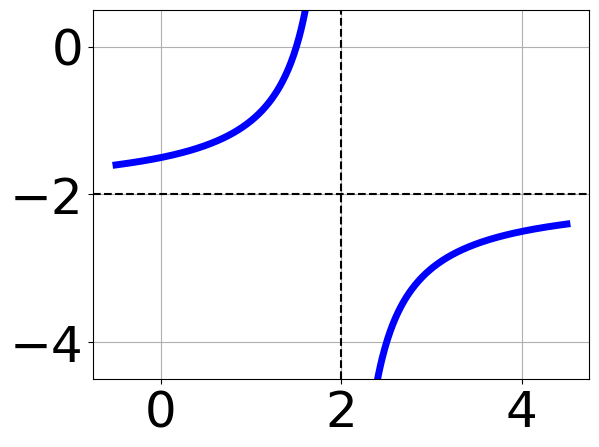
\includegraphics[width = 0.3\textwidth]{../Figures/rationalEquationToGraphDB.png}\end{multicols}\item None of the above.
\end{enumerate} }
\litem{
Solve the rational equation below. Then, choose the interval(s) that the solution(s) belongs to.\[ \frac{-45}{-72x + 18} + 1 = \frac{-45}{-72x + 18} \]\begin{enumerate}[label=\Alph*.]
\item \( x_1 \in [-0.7, -0.1] \text{ and } x_2 \in [0.25,4.25] \)
\item \( x \in [-0.7,-0.1] \)
\item \( \text{All solutions lead to invalid or complex values in the equation.} \)
\item \( x \in [-0.75,1.25] \)
\item \( x_1 \in [0.1, 0.9] \text{ and } x_2 \in [0.25,4.25] \)

\end{enumerate} }
\litem{
Determine the domain of the function below.\[ f(x) = \frac{4}{9x^{2} -21 x + 12} \]\begin{enumerate}[label=\Alph*.]
\item \( \text{All Real numbers except } x = a, \text{ where } a \in [0.73, 1.27] \)
\item \( \text{All Real numbers except } x = a \text{ and } x = b, \text{ where } a \in [0.73, 1.27] \text{ and } b \in [1.07, 1.91] \)
\item \( \text{All Real numbers except } x = a, \text{ where } a \in [8.88, 9.19] \)
\item \( \text{All Real numbers.} \)
\item \( \text{All Real numbers except } x = a \text{ and } x = b, \text{ where } a \in [8.88, 9.19] \text{ and } b \in [11.76, 12.03] \)

\end{enumerate} }
\litem{
Solve the rational equation below. Then, choose the interval(s) that the solution(s) belongs to.\[ \frac{-6x}{3x + 6} + \frac{-5x^{2}}{21x^{2} +57 x + 30} = \frac{-5}{7x + 5} \]\begin{enumerate}[label=\Alph*.]
\item \( x_1 \in [0.48, 0.9] \text{ and } x_2 \in [-1.97,4.03] \)
\item \( \text{All solutions lead to invalid or complex values in the equation.} \)
\item \( x \in [-1.35,-0.83] \)
\item \( x \in [-0.88,-0.71] \)
\item \( x_1 \in [0.48, 0.9] \text{ and } x_2 \in [-5,-1] \)

\end{enumerate} }
\litem{
Determine the domain of the function below.\[ f(x) = \frac{4}{18x^{2} +21 x -15} \]\begin{enumerate}[label=\Alph*.]
\item \( \text{All Real numbers.} \)
\item \( \text{All Real numbers except } x = a, \text{ where } a \in [-4.67, -0.67] \)
\item \( \text{All Real numbers except } x = a \text{ and } x = b, \text{ where } a \in [-4.67, -0.67] \text{ and } b \in [-0.5, 1.5] \)
\item \( \text{All Real numbers except } x = a, \text{ where } a \in [-17, -12] \)
\item \( \text{All Real numbers except } x = a \text{ and } x = b, \text{ where } a \in [-17, -12] \text{ and } b \in [15, 20] \)

\end{enumerate} }
\litem{
Solve the rational equation below. Then, choose the interval(s) that the solution(s) belongs to.\[ \frac{-6x}{-6x -4} + \frac{-7x^{2}}{-30x^{2} -2 x + 12} = \frac{3}{5x -3} \]\begin{enumerate}[label=\Alph*.]
\item \( \text{All solutions lead to invalid or complex values in the equation.} \)
\item \( x \in [1.09,1.68] \)
\item \( x_1 \in [-1.53, -0.16] \text{ and } x_2 \in [-1.8,-0.3] \)
\item \( x_1 \in [-1.53, -0.16] \text{ and } x_2 \in [0.7,1.5] \)
\item \( x \in [0.46,1.06] \)

\end{enumerate} }
\litem{
Choose the equation of the function graphed below.
\begin{center}
    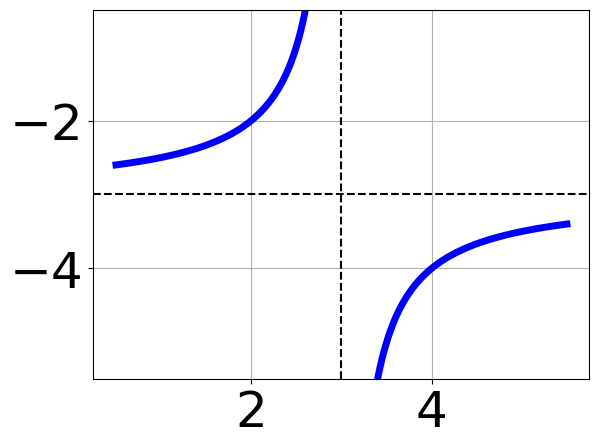
\includegraphics[width=0.5\textwidth]{../Figures/rationalGraphToEquationB.png}
\end{center}
\begin{enumerate}[label=\Alph*.]
\item \( f(x) = \frac{1}{(x + 3)^2} - 3 \)
\item \( f(x) = \frac{1}{x + 3} - 3 \)
\item \( f(x) = \frac{-1}{x - 3} - 3 \)
\item \( f(x) = \frac{-1}{(x - 3)^2} - 3 \)
\item \( \text{None of the above} \)

\end{enumerate} }
\litem{
Choose the equation of the function graphed below.
\begin{center}
    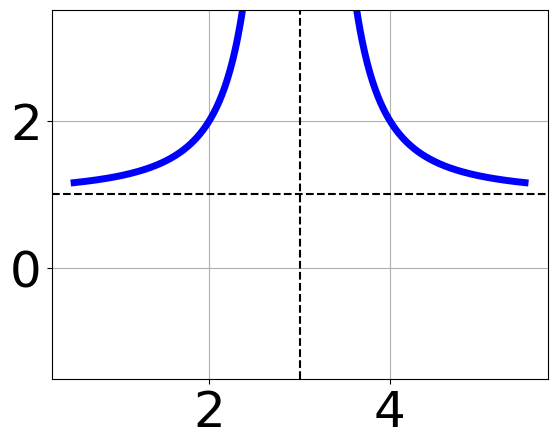
\includegraphics[width=0.5\textwidth]{../Figures/rationalGraphToEquationCopyB.png}
\end{center}
\begin{enumerate}[label=\Alph*.]
\item \( f(x) = \frac{1}{x - 3} + 1 \)
\item \( f(x) = \frac{-1}{(x + 3)^2} + 1 \)
\item \( f(x) = \frac{-1}{x + 3} + 1 \)
\item \( f(x) = \frac{1}{(x - 3)^2} + 1 \)
\item \( \text{None of the above} \)

\end{enumerate} }
\end{enumerate}

\end{document}